\documentclass[
  captions=tableheading,
  bibliography=totoc, 
  titepage=firstiscover,
]{scrartcl}

\usepackage{blindtext} %neuer input

\usepackage{longtable} % Tabellen über mehrere Seiten

\usepackage[utf8]{inputenc} %neuer input

\usepackage{scrhack}

\usepackage[aux]{rerunfilecheck} %Warnung falls nochmal kompiliert werden muss

\usepackage{fontspec} %Fonteinstellungen

\recalctypearea{}

\usepackage[main=ngerman]{babel} %deutsche Spracheinstellung

\usepackage{ragged2e} %neuer input

\usepackage{amsmath, nccmath}

\usepackage{amssymb} %viele mathe Symbole

\usepackage{mathtools} %Erweiterungen für amsmath


\DeclarePairedDelimiter{\abs}{\lvert}{\rvert}
\DeclarePairedDelimiter{\norm}{\lVert}{\rVert}

\DeclarePairedDelimiter{\bra}{\langle}{\rvert}
\DeclarePairedDelimiter{\ket}{\lvert}{\rangle}

\DeclarePairedDelimiterX{\braket}[2]{\langle}{\rangle}{
#1 \delimsize| #2
}

\NewDocumentCommand \dif {m}
{
\mathinner{\symup{d} #1}
}


\usepackage[
  math-style=ISO,
  bold-style=ISO,
  sans-style=italic,
  nabla=upright,
  partial=upright,
  warnings-off={
    mathtools-colon,
    mathtools-overbracket,
  },
]{unicode-math}

\setmathfont{Latin Modern Math}
\setmathfont{XITS Math}[range={scr, bfscr}]
\setmathfont{XITS Math}[range={cal, bfcal}, StylisticSet=1]


\usepackage[
  locale=DE,
  separate-uncertainty=true,
  per-mode=reciprocal,
  output-decimal-marker={,},
]{siunitx}

\usepackage[autostyle]{csquotes} %richtige Anführungszeichen

\usepackage{xfrac}

\usepackage{float}

\floatplacement{figure}{htbp}

\floatplacement{table}{htbp}

\usepackage[ %floats innerhalb einer section halten
  section,   %floats innerhalb er section halten
  below,     %unterhalb der Section aber auf der selben Seite ist ok
]{placeins}

\usepackage[
  labelfont=bf,
  font=small,
  width=0.9\textwidth,
]{caption}

\usepackage{subcaption} %subfigure, subtable, subref

\usepackage{graphicx}

\usepackage{grffile}

\usepackage{booktabs}

\usepackage{microtype} %Verbesserungen am Schriftbild

\usepackage[
backend=biber,
]{biblatex}

\addbibresource{../lit.bib}

\usepackage[ %Hyperlinks im Dokument
  german,
  unicode,
  pdfusetitle,
  pdfcreator={},
  pdfproducer={},
]{hyperref}

\usepackage{bookmark}

\usepackage[shortcuts]{extdash}

%\usepackage{warpcol}


\begin{document}
    \title{ATP Übungsblatt 5}
    \author{  
    Tobias Rücker\\
    \texorpdfstring{\href{mailto:tobias.ruecker@tu-dortmund.de}{tobias.ruecker@tu-dortmund.de}
    \and}{,} 
    Paul Störbrock\\
    \texorpdfstring{\href{mailto:paul.stoerbrock@tu-dortmund.de}{paul.stoerbrock@tu-dortmund.de}}{}
    }
\maketitle
\center{\Large Abgabegruppe: \textbf{Mittw. 10-12 Uhr}}
\thispagestyle{empty}

\newpage
\tableofcontents
\thispagestyle{empty}
\newpage

\setcounter{page}{1}

\section{Aufgabe 13}

    \begin{figure}[H]
        \centering
        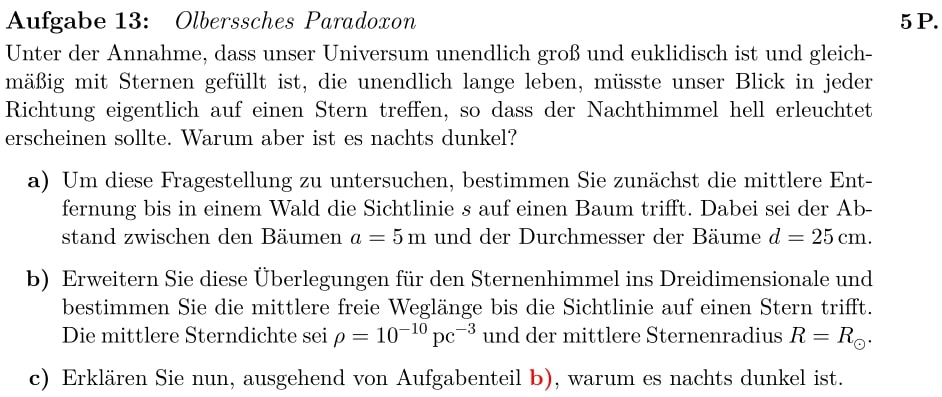
\includegraphics[width=\textwidth]{images/Aufgabe13.jpg}
        \label{fig:1}
    \end{figure}

\subsection{a)}

    \flushleft{Bei\;}\justifying der Wald-Analogie des Olbersschen Paradoxon wird die Formel der mittleren freien Weglänge im 2-Dimensionalen
    verwendet:
    \begin{align*}
        \lambda &= \frac{1}{\rho\cdot\sigma}
    \end{align*}
    \flushleft{Hierbei\;}\justifying ist $\rho$ die Baumdichte des Waldes und $\sigma$ der Wirkungsquerschnitt eines Baumes (\SI{25}{\centi\meter}).
    Um die Baumdichte bestimmen zu können, wird eine Fläche vorrausgesetzt. Hier wird eine Approximation der Fläche des Stadtwaldes von Dattel
    verwendet. Die Fläche des Lohbusches ist ungefähr:
    \begin{align*}
    \text{Länge} &= \text{\input{Länge.tex}}\\
    \text{Breite} &= \text{\input{Breite.tex}}\\
    \text{Fläche} &= \text{\input{Fläche.tex}}
    \intertext{
        \flushleft{Aus\;}\justifying der Fläche lässt sich über die Teilchenzahl $N$ die Baumdichte mithilfe von
    }
    \rho &= \frac{N}{A}
    \intertext{
        \flushleft{bestimmen.\;}\justifying Da die Baumverteilung als homogen bei einem Abstand von \SI{5}{\meter} angenommen wird,
        ist die Baumzahl $N$ hiermit:
    }
    N &= \frac{A}{25} = \text{\input{Baumzahl.tex}}
    \intertext{
        \flushleft{Die\;}\justifying Baumdichte und die daraus folgende Sichtweite sind damit:
    }
    \rho &= \text{\input{Baumdichte.tex}}\\
    \Rightarrow \lambda &= \frac{1}{\rho\cdot\sigma} = \text{\input{lambda.tex}}
    \end{align*}


\subsection{b)}

    \flushleft{Wird\;}\justifying das Analogon aus Aufgabenteil a) auf den 3-dimensionalen Raum des Universums angewandt, bei einer 
    mittleren Sternendichte von $\rho = 10^{-10}\text{pc}^{-3}$ und einem mittleren Sternenradius $R=R_{\odot}$, ergibt
    sich für die mittlere Entfernung:
    \begin{align*}
        \lambda &= \frac{1}{\rho \sigma} \qquad \text{mit}\; \sigma = \pi\cdot R_{\odot}^2 = \text{\input{sigma_13b.tex}}\\
        \Rightarrow\lambda &= \text{\input{lambda_13b.tex}}
        \intertext{
            \flushleft{In\;}\justifying Parsec ergibt das:
        }
        \Rightarrow\lambda &= \text{\input{lambda_13b_parsec.tex}}
    \end{align*}

\subsection{c)}

    \flushleft{Der\;}\justifying Grund, dass der Nachthimmel dunkel ist, liegt an der falschen Annahme des Paradoxons, dass das Universum 
    unendlich alt ist. Mit einem geschätzten Alter von 15 milliarden Jahren, hat das momentane Universum einen Radius von ca. 15 milliarden
    Lichtjahren. Wird nun die mittlere freie Weglänge aus b) in Lichtjahre umgerechnet, ergibt sich:
    \begin{align*}
        \lambda &= \text{\input{lambda_13c.tex}}\\
        \frac{15\cdot 10^9\text{ly}}{\text{\input{lambda_13c}}\cdot 100} &= \text{\input{percent.tex}}
    \end{align*}
    \flushleft{Aus\;}\justifying dem Prozentsatz vom Alter des Universums über der mittleren freien Weglänge lässt sich schließen,
    dass das Licht der Sterne außerhalb des observablen Universums, im Falle eines unendlichen Universums, nicht die Zeit hatte,
    uns zu erreichen. 


\section{Aufgabe 14}

    \begin{figure}[H]
        \centering
        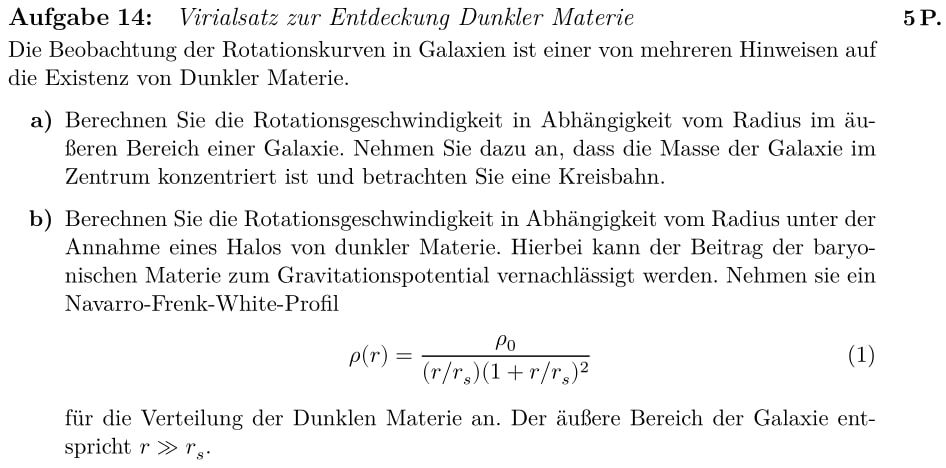
\includegraphics[width=\textwidth]{images/Aufgabe14ab.jpg}
        \label{fig:2}
    \end{figure}

    \begin{figure}[H]
        \centering
        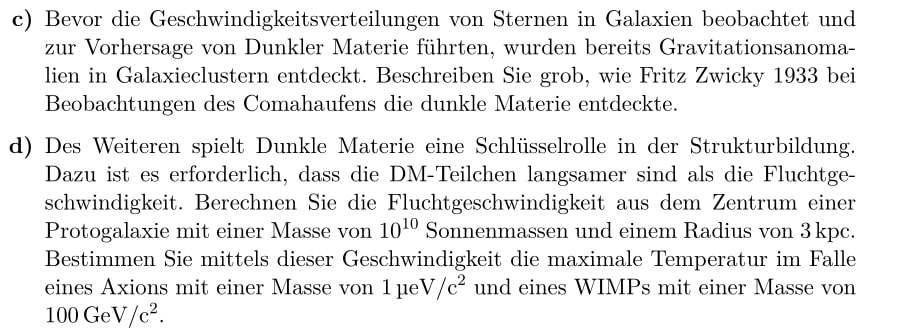
\includegraphics[width=\textwidth]{images/Aufgabe14cd.jpg}
        \label{fig:3}
    \end{figure}

\subsection{a)}
\begin{align}
    m \frac{v^2}{r} &= \frac{GMm}{r^2}\\
    v &= \sqrt{\frac{GM}{r}}
\end{align}


\subsection{b)}
\begin{align}
    M &= \int_0^{2 \pi} \int_0^{\pi} \int_0^r r^{'2} \sin \theta \rho (r') \,\dif{r'} \\
    &= 4 \pi \int_0^r r^{'2} \frac{\rho_0}{(\frac{r'}{r_s})(1+\frac{r'}{r_S})^2} \dif{r'} \\
    &= 4 \pi \rho _0 r_s \int_0^r \frac{r'}{(1+\frac{r'}{r_s})^2} \,\dif{r'} \\
    &= 4 \pi \rho _0 r_s^3 \int_0^r \frac{r'}{(r_s+r')^2} \,\dif{r'}\\
    \intertext{
        Substitution:
    }
    r_s+r'&=u\\
    \frac{\dif{u}}{\dif{r'}} &= 1\\
    \intertext{
        weiter
    }
    &= 4 \pi \rho _0 r_s^3 \int_{r_s}^{r_s +r} \frac{u-r_s}{u^2} \dif{u}\\
    &= 4 \pi \rho _0 r_s^3 \int_{r_s}^{r_s+r} \frac{1}{u} - \frac{r_s}{u^2} \dif{u} \\
    &= 4 \pi \rho _0 r_s^3 (\ln(u)+ \frac{r-s}{u} )\vert _{r_s}^{r_s+r}\\
    &= 4 \pi \rho _0 r_s^3 (\ln(\frac{r_s+r}{r_s})-\frac{r}{r+r_s})
    \intertext{
        Für M in Aufgabenteil a einsetzen
    }
    \Rightarrow v &= \sqrt{\frac{G 4 \pi r_s^3 (\ln(\frac{r_s+r}{r_s}-\frac{r}{r+r_s}))}{r}}
\end{align}


\subsection{c)}
\flushleft{Fritz\,}\justifying Zwicky hatte die Relativbewegungen von Galaxien im Coma-Haufen betrachtet,
da viel Masse schnelle Bewegung der Galaixien hervorruft. Über die Bestimmung
der Geschwindigkeitsdispersion und das Virialtheorem lässt sich dann die Masse des Coma-Haufens berechnen.
Das Masse-Leuchtkraft-Verhältnis für den Coma-Haufen ergab sich zu $250 M_{\odot}/L_{\odot} $. Für typische Sterne
in Galaxien gilt ein Verhältnis von $2,5 M_{\odot}/L_{\odot} $

\subsection{d)}


\section{Aufgabe 15}

    \begin{figure}[H]
        \centering
        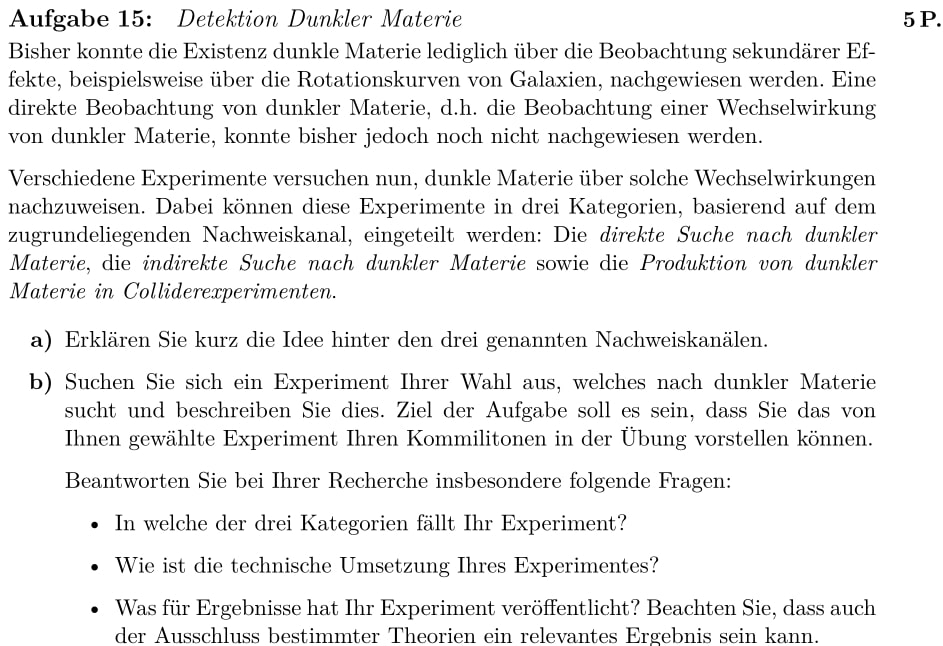
\includegraphics[width=\textwidth]{images/Aufgabe15.jpg}
        \label{fig:4}
    \end{figure}

\subsection{a)}

    \flushleft{Direkte\;}\justifying Suche:\\
    Da dunkle Materie (DM) beim Wechselwirken mit normaler Materie (Materie des standard Modells) Energie in Form eines Lichtquants abgibt, kann dieser Lichtquant
    mithilfe von Photomultipliern (ähnlich derer des ICE Cubes) detektiert werden.

    \flushleft{Indirekte\;}\justifying Suche:\\
    Detektion der Emission eines $\gamma$-Quants, welcher durch die Annihilation des DM Teilchens entsteht. Zum Beispiel mit $\gamma$-Teleskope.

    \flushleft{Produktion:\;}\justifying\\
    DM Teilchen können künstlich erzeugt werden, indem standard Modell Teilchen mit außreichend Geschwindigkeit kollidieren. Das DM Teilchen selbst kann anschließend
    durch die Wechselwirkung nachgewiesen werden. Zum Beispiel im LHC.

\subsection{b)}

    \flushleft{XENON1T\;}\justifying Dark Matter Project \footnote{Raphael Lang, XENON1T probes deeper into Dark Matter WIMPs, with 1300 kg of cold Xe atoms, 
    2018, \url{http://www.xenon1t.org/}, Online; besucht am 1. Juni 2020}:\\
    In welche der drei Kathegorien fällt Ihr Experiment?\\
    Direkte Suche

    \flushleft{Wie\;}\justifying ist die technische Umsetzung Ihres Experiments?\\
    Das Experiment besteht aus einem \SI{62}{\kilo\gram} Behälter, welcher mit einer Xenonflüssigkeit (Ziel) und einem Xenongas gefüllt ist. Am Deckel und am Boden des
    Behälters befinden sich Photomultiplierrohre (PMT). Die PMT am Boden messen ein schimmerndes Licht (S1) in der Xenonflüssigkeit, welches durch einem, in das Ziel einfallende 
    Teilchen, emittiert wird. Außerdem befindet sich im Xenongas eine Anode und nahe dem Boden in der Xenonflüssigkeit die dazugehörige Kathode. Das elektrische Feld beschleunigt 
    die surch Ionisatoin freigesetzten Elektronen zur Kathode (zum Gas), wo sie einen zweiten Lichtimpuls abgeben (S2), welcher abermals von den PMT gemessen wird. Die Diskrepanz der beiden Messungen lässt auf 
    die vertikale Position der Wechselwirkung in der Xenonflüssigkeit schließen. Die zweite Messung S2 gibt außerdem die horizontale Komponente, wodurch die Lokalisation des 
    Ereignisses im 3-dim. Raum ermöglicht wird.\\
    Das XENON1T Experiment betrachtet weakly interacting massive particles (WIMPs) Wechselwirkungen mit normaler Materie. Hier wird ein Zustand ohne nuklearen Spin angenommem. 
    Die WIMPs sind deshalb von Interesse, da WIMPs als potentielle Kandidaten für DM in Frage kommen. 

    \flushleft{Was\;}\justifying für Ereignisse hat Ihr Experiment veröffentlicht?\\
    XENON1T hat das Wechselwirkungslimit eines WIMPs über eine Zeitspanne von einem Jahr gemessen. Das XENON1T Experiment liefert außerdem mitunter die saubersten Messungen, da
    die Hintergrundstrahlung selten (ca.630 Events pro Jahr) gemessen wird. Über ein Jahr wurden zwei Events im Zentrum des Behälters erwartet, jedoch keine gemessen. XENON1T 
    ist der Vorgänger des neuen Experiments XENONnT, welches einen 4-fach größeren Behälter und einer 10-fach geringeren Eventrate aufweist.

\end{document}